\documentclass{mwrep}

% Polskie znaki
\usepackage{polski}
\usepackage[utf8]{inputenc}
\usepackage[T1]{fontenc}
\usepackage{lmodern}
\usepackage{indentfirst}

% Strona tytułowa
\usepackage{pgfplots}
\usepackage{siunitx}
\usepackage{paracol}

% Pływające obrazki
\usepackage{float}
\usepackage{svg}
\usepackage{graphicx}

% table of contents refs
\usepackage{hyperref}
\usepackage{cleveref}
\usepackage{booktabs}
\usepackage{listings}

\restylefloat{table}



\SendSettingsToPgf
\title{\bf Projekt układu regulacji obiektu grzejąco-chłodzącego\vskip 0.1cm}
\author{Krystian Guliński \and Jakub Sikora \and Konrad Winnicki}
\date{\today}
\pgfplotsset{compat=1.15}	
\begin{document}

\makeatletter
\renewcommand{\maketitle}{\begin{titlepage}
		\begin{center}{
				\LARGE {\bf Politechnika Warszawska}}\\
			\vspace{0.4cm}
			{\LARGE {\bf Wydział Elektroniki i Technik Informacyjnych}}\\
			\vspace{5cm}
			{\bf \LARGE \mbox{Systemy DCS i SCADA} \vskip 0.1cm}
		\end{center}
		\vspace{0.1cm}

		\begin{center}
			{\bf \LARGE \@title}
		\end{center}

		\vspace{10cm}
		\begin{paracol}{2}
			\addtocontents{toc}{\protect\setcounter{tocdepth}{1}}
			\subsection*{Zdający:}
			\bf{ \Large{ \noindent\@author \par}}
			\addtocontents{toc}{\protect\setcounter{tocdepth}{2}}

			\switchcolumn \addtocontents{toc}{\protect\setcounter{tocdepth}{1}}
			\subsection*{Prowadzący:}
			\bf{\Large{\noindent dr inż. Sebastian \\ Plamowski}}
			\addtocontents{toc}{\protect\setcounter{tocdepth}{2}}

		\end{paracol}
		\vspace*{\stretch{6}}
		\begin{center}
			\bf{\large{Warszawa, \@date\vskip 0.1cm}}
		\end{center}
	\end{titlepage}
}
\makeatother
\maketitle

\tableofcontents

\chapter{Obiekt regulacji}
\label{ObiektRegulacji}

\section{Opis obiektu termicznego}
\label{ObiektTermiczny}
Obiektem regulacji jest laboratoryjne stanowisko chłodząco-grzejące. Jest to obiekt cieplny, 
w którym jako elementy grzewcze wykorzystano rezystory mocy, w specjalnych obudowach dobrze odprowadzających
wytworzone ciepło. Do chłodzenia wykorzystano wysokoobrotowe
wentylatory. Zastosowano czujniki temperatury z magistralą danych
OneWire – oznaczenia. Dodatkowo wykorzystano płytę pomiarową
służącą do odczytu wartości prądu oraz napięcia. Urządzenie może pracować w trzech trybach komunikacji: poprzez
dedykowany protokół komunikacyjny przy użyciu standardu USB,
protokół MODBUS RTU oraz standard napięciowy RS485 lub poprzez
standard sygnałów analogowych 0-10V podłączając regulator przy użyciu złączy
śrubowych. Użytkownik ponadto ma możliwość zmiany charakteru obiektu, w tym celu
zamontowana została fizyczna przegroda. Wykorzystana jest ona do oddzielenia dwóch
strumieni powietrza wentylatora lewego i prawego, dzięki czemu można zredukować
zakłócenia wynikające z mieszania się strumieni. W ćwiczeniu, obiekt laboratoryjny
został znacząco uproszczony do przypadku jednowymiarowego. Wartością regulowaną była
wartość temperatury odczytana na czujniku temperatury T1. Sterowanie temperaturą odbywało się 
za pomocą grzałki G1. W ramach utrudnienia, na obiekt działało zakłócenie w postaci wentylatora W1.

\section{Zebranie odpowiedzi skokowej}
\label{OdpowiedzSkokowa}
Pierwszym krokiem do zamodelowania obiektu było wyznaczenie jego odpowiedzi skokowych. Przebiegi otrzymanych odpowiedzi skokowych można zobaczyć na tle wyznaczonych na ich podstawie modelów w kolejnym podrozdziale.
Głównym problemem było zapewnienie odpowiednich warunków pomiarów. Należało w tym celu zadbać o mały ruch ludzi wokół obiektu, a szczególnie pilnować otwierania i zamykania drzwi do laboratorium.
Pozyskano dwa typy odpowiedzi skokowych - reakcję na skok sterowania grzałką oraz reakcję na skok sterowania wiatraka(zakłócenie). Pozwolą nam one na odpowiednie określenie parametrów obiektu w celu jego dalszej identyfikacji i regulacji.


\section{Proces modelowania obiektu}
\label{ModelowanieObiektu}
Przy pomocy zebranej odpowiedzi skokowej obiektu, za pomocą Matlaba dokonaliśmy identyfikacji 
modelu jednoinercyjnego. Pomimo że obiekt fizycznie jest co najmniej dwuinercyjny, zdecydowaliśmy się na 
przybliżenie go pojedynczą inercją w celu uproszczenia struktury regulacji. \\
\indent Do przeprowadzania identyfikacji wykorzystaliśmy funkcję \texttt{tfest}, która na podstawie 
przebiegów czasowych wyznacza parametry zadanej transmitancji. 

Otrzymany model obiektu:

\[model\_obiektu(s) = \frac{0.00395}{s + 0.008166}\]

\begin{figure}[H]
\centering
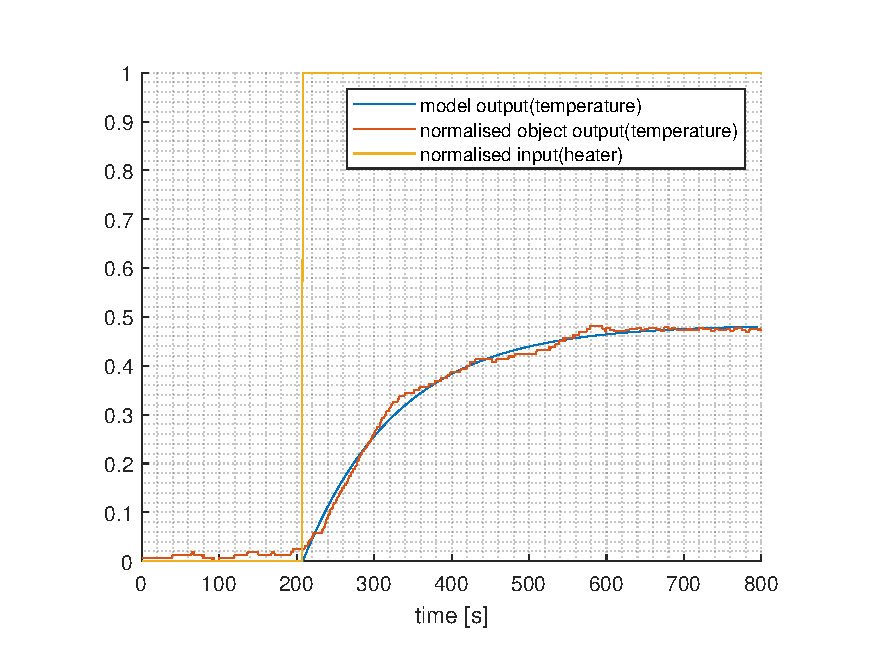
\includegraphics[scale=0.8]{materialy/krystian_plots/wykresik_model_obiekt.pdf}
\caption{Porownanie wyjscia modelu z obiektem}
\end{figure}

\section{Proces modelowania zakłóceń}
\label{ModelowanieZaklocen}
Przy pomocy zebranej odpowiedzi skokowej obiektu w trakcie reakcji na zmianę zakłóceń byliśmy w stanie w analogiczny sposób wyznaczyć również model zakłóceń, który potem będzie przydatny przy odsprzęganiu zakłóceń.

Otrzymany model zakłóceń:

\[model\_zaklocen(s) = \frac{-0.0003625}{s + 0.01105}\]

\begin{figure}[H]
\centering
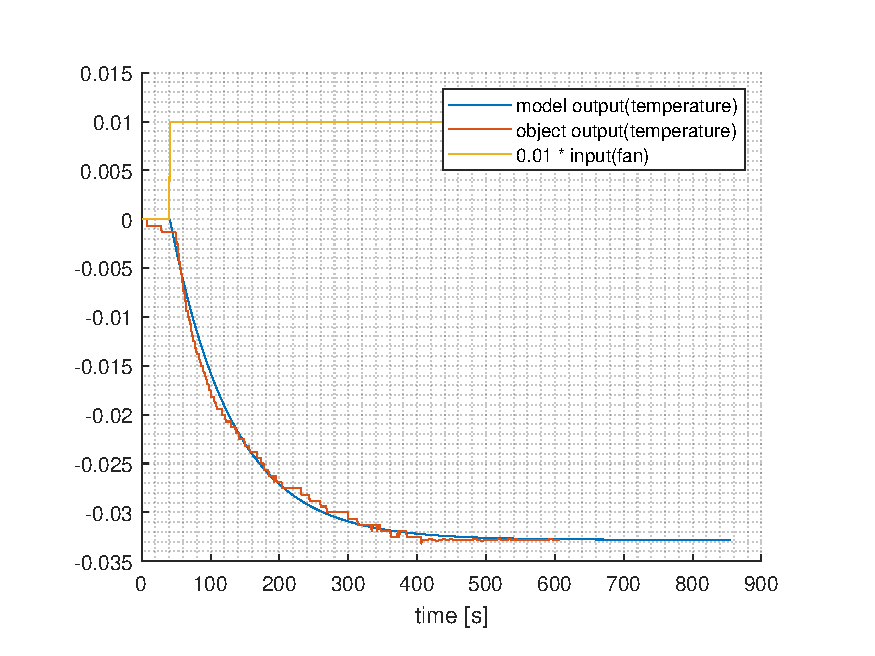
\includegraphics[scale=0.8]{materialy/krystian_plots/wykresik_zaklocenia.pdf}
\caption{Porownanie wyjscia modelu z obiektem w sytuacji badania zakłóceń}
\end{figure}


\chapter{Układ regulacji}
\label{UkladRegulacji}

Ze względu na możliwość pomiaru zakłóceń do regulacji obiektu został użyty schemat sterowania obiektu regulatorem PID (realizacja OVATION) z kompensowaniem zakłóceń (feedforward) w strukturze otwartej przedstawiony na wykładzie z przedmiotu DCS.

\section{Algorytm PID}
\label{PID}

Parametry regulatora PID zostały dobrane na podstawie modelu wyznaczonego w poprzedniej części projektu. W tym celu został użyty PID Tuner dostępny w środowisku MATLAB.

Równanie regulatora PIDF dostępnego w środowisku MATLAB:

\vspace{2mm}
$PIDF_{MATLAB}(s) = K _ { p } + \frac { K _ { i } } { s } + \frac { K _ { d } s } { T _ { f } s + 1 }$
\vspace{3mm}

Równanie regulatora PID dostępnego w systemie Ovation:
\vspace{2mm}

$PID_{ovation}(s) = K _ { p } + \frac { 1 } {  T _ { i } s } + \frac { K _ { d } s } { T _ { f } s + 1 }$
\vspace{3mm}

Jak widać różnica jest znikoma, aby dostosować parametry otrzymane z PID Tuner należy obliczyć wartość parametru Ti według wzoru $T_{i} = \frac{1}{K_{i}}$

\begin{figure}[H]
\centering
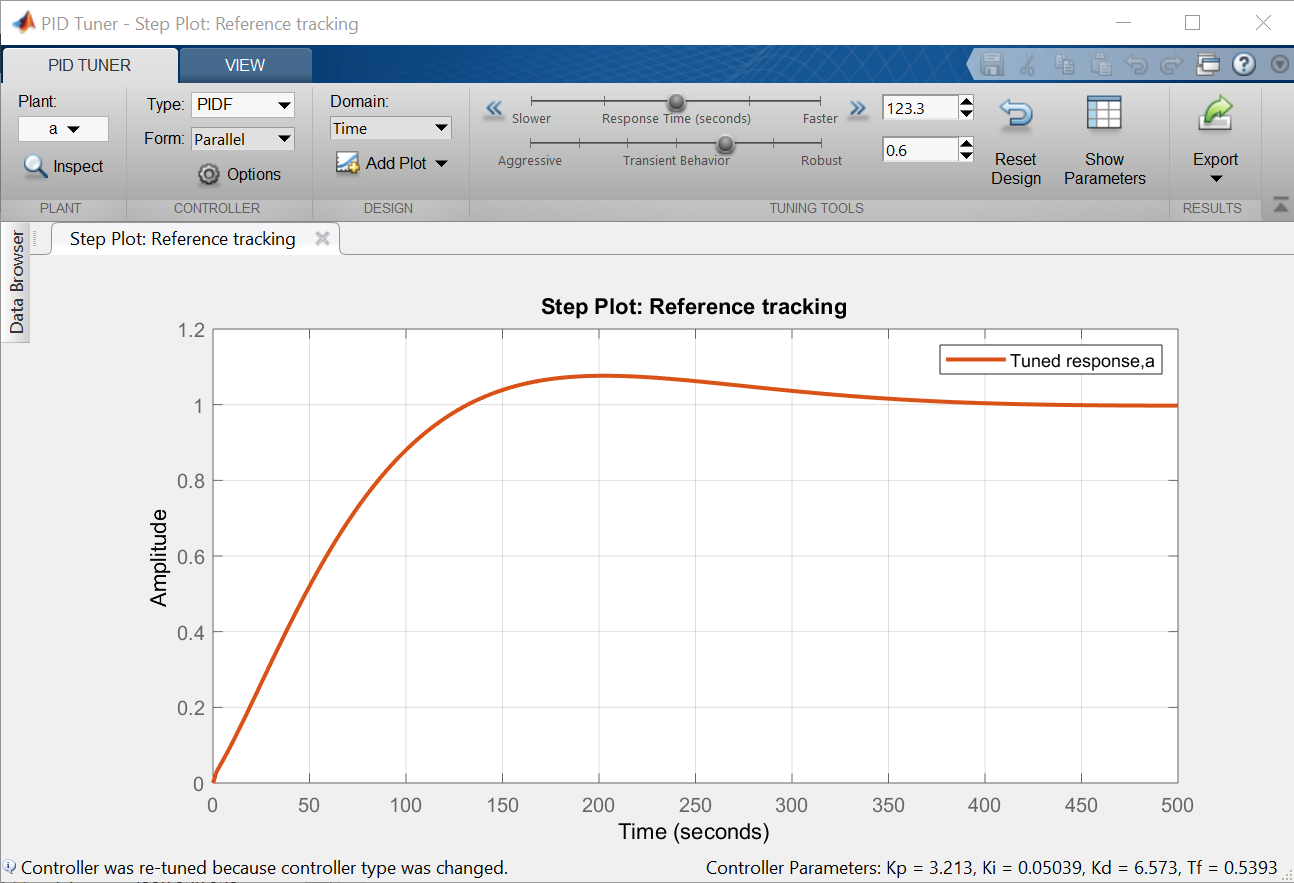
\includegraphics[scale=0.4]{materialy/krystian_plots/pid_tuner.png}
\caption{Widok procesu strojenia regulatora PID w PID Tunerze}
\end{figure}

Otrzymane parametry:

\begin{table}[H]
\begin{tabular}{l|cccl}
Regulator    & Kp     & Ki/Ti        & Td     & Tf      \\ \hline
PIDF\_MATLAB & 3.2078 & Ki = 0.0502  & 6.3794 & 0.54035 \\
PID\_OVATION & 3.2079 & Ti = 19.8977 & 6.3794 & 0.54035
\end{tabular}
\end{table}
\newpage
\section{Człon odsprzęgający}
\label{Odsprzeganie}
Do obliczenia transmitancji odsprzęgania wykorzystamy wcześniej wyznaczone modele obiektu i zakłóceń, następnie zostanie ona przekształcona w celach implementacji w systemie OVATION.
Transmitancja wykorzystywana do odsprzęgania wygląda następująco:

\vspace{3mm}
$G_{odsp}(s) = \frac{-G_{z}(s)}{G_{o}(s)} = \frac{0.0003626 s + 2.969 \cdot 10^{-6}}{0.003956 s + 4.374 \cdot 10^{-5}}$

\vspace{3mm}
$G_{odsp}(s) = 0.0679 \cdot \frac{122.1315s + 1}{90.4449s +1}$

\vspace{3mm}

Taką transmitancje możemy zrealizować elementem LEADLAG dostępnym w systemie OVATION. Parametry tego elementu zostały wyciągnięte z przekształconej transmitancji i wpisane do tabelki w odpowiadające im miejsca.

\begin{table}[H]
\begin{tabular}{l|l}
Parametr LEADLAG & Wartość  \\ \hline
GAIN             & 0.0679   \\
LEAD             & 122.1315 \\
LAG              & 90.4449 
\end{tabular}
\end{table}

\chapter{Implentacja w systemie OVATION}
\label{OVATION}

\section{Control sheet}
\label{ControlSheet}

Korzystając z programu Control Builder i zawartych w nim bloków funkcyjnych takich jak PID, LEAD LAG, TRANSFER, SUM, IN i OUT zaimplementowano regulator PID z odsprzęganiem zakłóceń.  Wartością regulowaną(PV) była temperatura T1, wartością sterowaną(MV) było wysterowanie grzałki G1, a zakłóceniem(DV) był wydatek wentylatora W4.

Do wejść regulatora PID doprowadzono sygnał z termometru T1 oraz wartość zadaną temperatury. Wyjście regulatora poprzez sumator steruje grzałką G1. Do sumatora dołączono również sygnał odsprzęgający zakłócenie od wentylatora W4.


\begin{figure}[H]
\centering
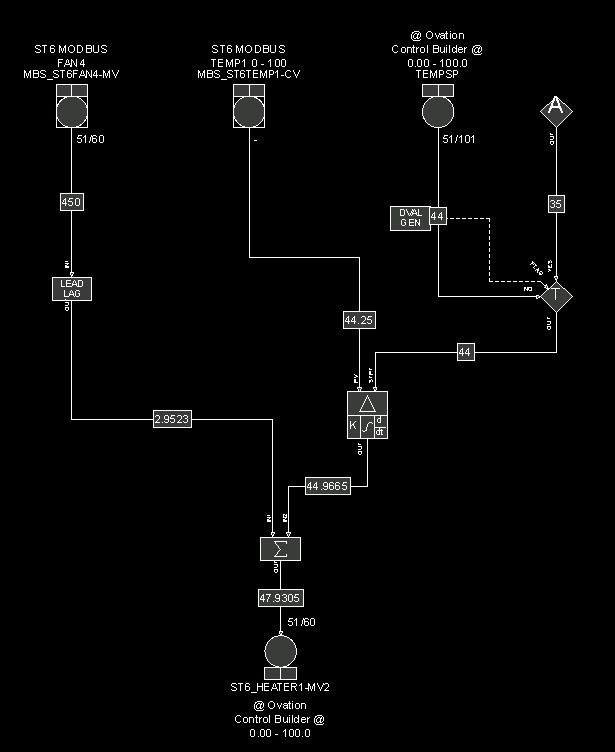
\includegraphics[scale=0.4]{materialy/regulator_cutout.png}
\caption{Widok control sheet'u w Signal Diagram Viewer}
\end{figure}

\section{Użyte algorymty}
\label{AlgorytmyOVATION}

W implementacji zastosowano bloki funkcyjne:
\begin{itemize}
  \item PID – regulator PID
  \item LEAD LAG – blok realizujący transmitancję o określonych parametrach
  \item SUM – blok sumujący wartości sygnałów na jego wejściach
  \item TRANSFER – blok realizujący przełączanie gałęzi układu regulacji, pozwolił na wybór źródła wartości zadanej temperatury
  \item DVALGEN – źródło sygnału binarnego, zastosowany do przełączania bloku
  \item IN – wejście sygnałów do control sheet
  \item OUT – wyjście sygnałów z control sheet
\end{itemize}
 
\chapter{Testy układu regulacji}
\label{Testy}

Po zaimplementowaniu regulatora PID rozpoczęto testy układu regulacji mające na celu określenie jakości regulacji w sytuacjach zmian wartości zadanej temperatury oraz zmian wartości zakłócenia.

Wykonano serie skoków wartości zadanej temperatury i skoków wartości zakłócenia rejestrując zachowanie regulatora i obiektu regulacji.

Testy wykazały zadowalające osiągi układu regulacji, zaobserwowane reakcje regulatora na  skoki wartości zadanej oraz skoki zakłócenia pozwalają stwierdzić, że dobrany regulator bardzo dobrze spełnia założenia projektu. 


\section{Testy reakcji na zmianę wartości zadanej}
\label{TestyWewnetrzne}

\begin{figure}[H]
\centering
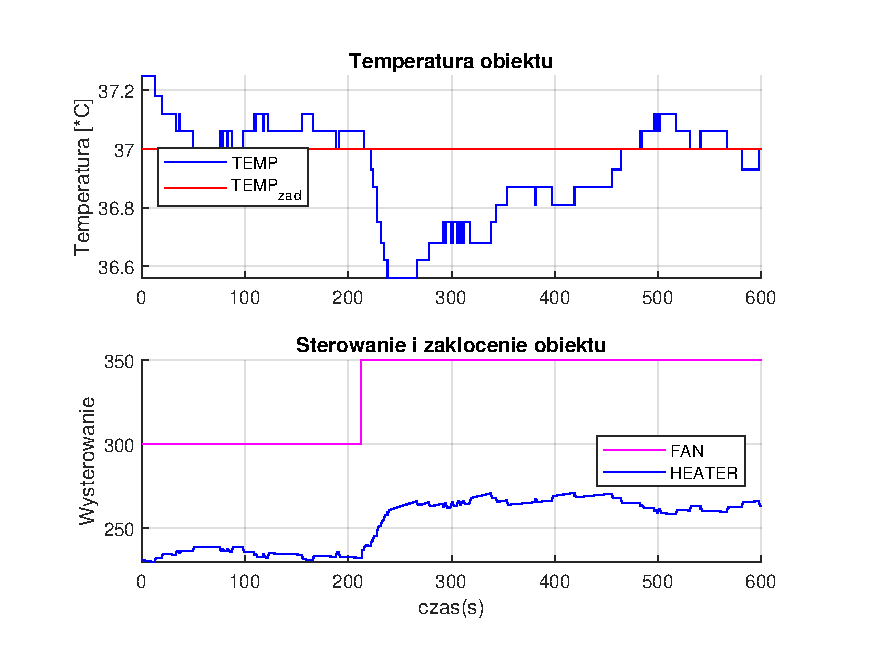
\includegraphics[scale=0.85]{materialy/krystian_plots/3035wiatrzakl.pdf}
\caption{Skok wartości zadanej z 30 na 35 stopni}
\end{figure}

\begin{figure}[H]
\centering
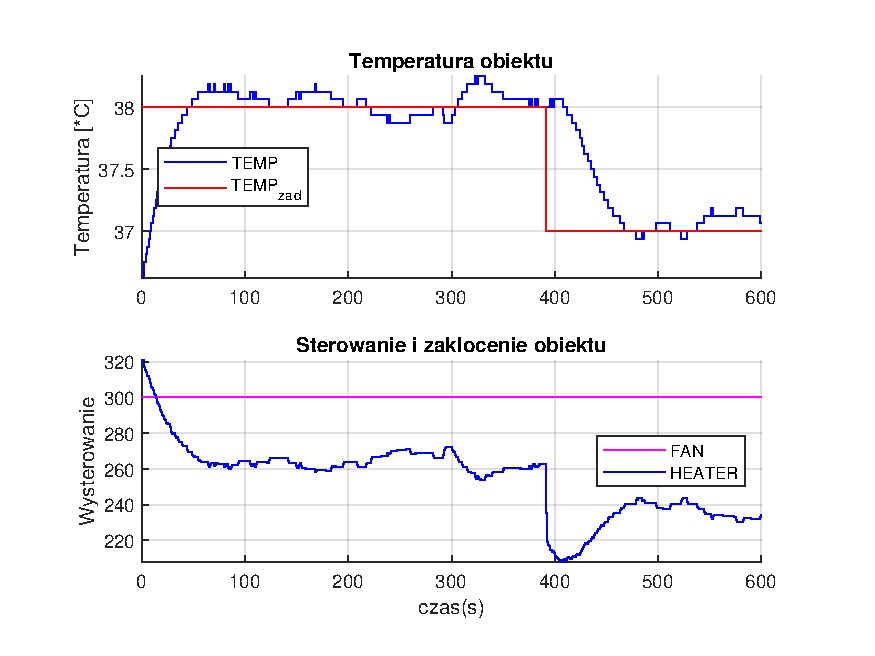
\includegraphics[scale=0.85]{materialy/krystian_plots/3837heater.pdf}
\caption{Skok wartości zadanej z 38 na 37 stopni}
\end{figure}

\section{Testy reakcji na zmianę wartości zakłóceń}
\label{Konkurs}

\begin{figure}[H]
\centering
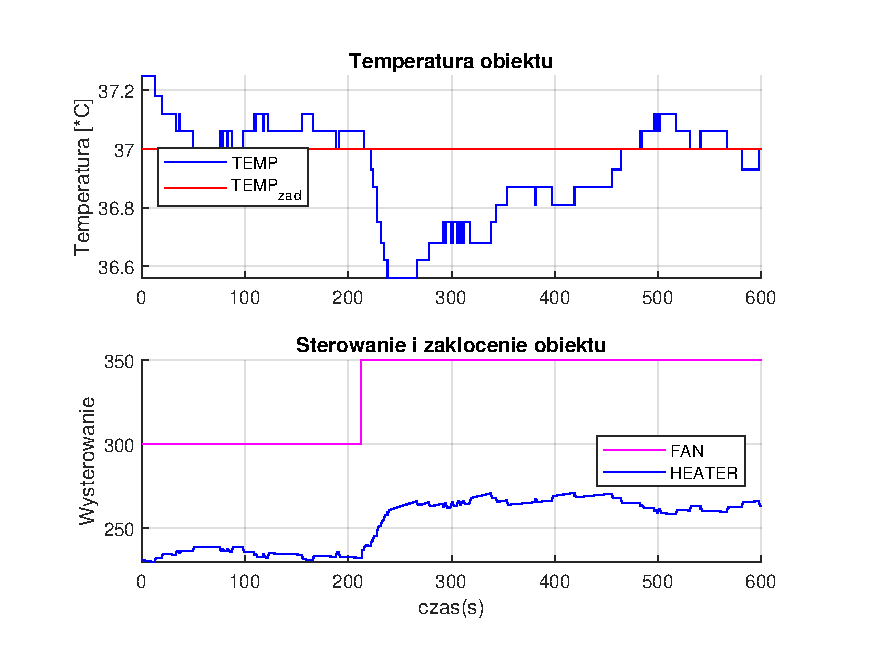
\includegraphics[scale=0.85]{materialy/krystian_plots/3035wiatrzakl.pdf}
\caption{Skok wartości sterowania wiatraka (zakłócenie) z 30 na 35 procent}
\end{figure}

\begin{figure}[H]
\centering
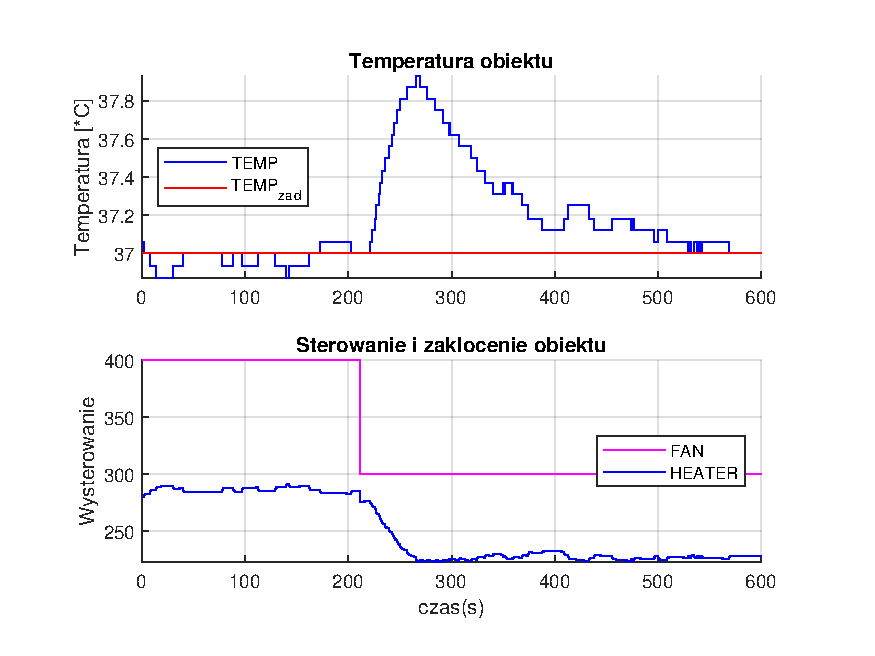
\includegraphics[scale=0.85]{materialy/krystian_plots/4030wiatrak.pdf}
\caption{Skok wartości sterowania wiatraka (zakłócenie) z 40 na 30 procent}
\end{figure}


\section{Konkurs pomiędzy grupami laboratoryjnymi}
\label{eeee}
Finałem projektu był przeprowadzony przez prowadzącego konkurs mający na celu wyłonienie najlepszego regulatora zaimplementowanego przez studentów. Oceną jakości regulacji w trakcie trwania konkursu było zliczanie błędu średniokwadratowego uchybu w chwilach gdy uchyb był większy od założonej wartości półstopnia Celsiusza.

Konkurs zakładał przełączenie sterowania wszystkich stanowisk na ten sam sygnał sygnał wartości zadanej temperatury oraz ten sam sygnał zakłócenia.  Po przełączeniu sterowań odczekano na stabilizację wszystkich obiektów, po czym wykonano skok wartości zadanej temperatury, odczekano na stabilizację i wykonano skok zakłócenia. 

W tak przeprowadzonym konkursie regulator z powyższego sprawozdania osiągnął trzecie miejsce.

\end{document}